
\begin{figure}[H]
\centering
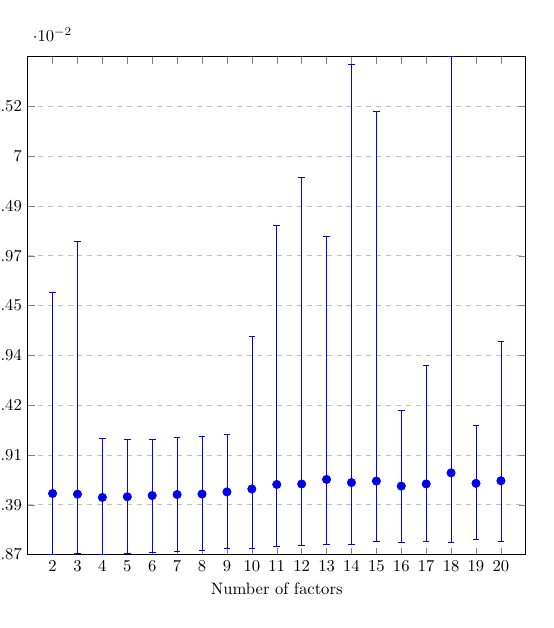
\begin{tikzpicture}[scale=0.6, trim axis left, trim axis right]
\begin{axis}[
    width=1\textwidth,
    height=1\textwidth,
    xlabel={Number of factors},
    ylabel={Time taken (s)},
    xmin=1.0, xmax=21.0,
    ymin=0.028721, ymax=0.080366,
    xticklabels={2, 3, 4, 5, 6, 7, 8, 9, 10, 11, 12, 13, 14, 15, 16, 17, 18, 19, 20},
    xtick={2, 3, 4, 5, 6, 7, 8, 9, 10, 11, 12, 13, 14, 15, 16, 17, 18, 19, 20},
    ytick={0.028721, 0.0338855, 0.03905, 0.0442145, 0.049379, 0.0545435, 0.059708, 0.0648725, 0.070037, 0.0752015},
    ymajorgrids=true,
    grid style=dashed,
]

\addplot+[
    blue,
    very thick,
    forget plot,
    only marks
    ]
    plot[
    very thick,
    error bars/.cd,
    y dir=plus,
    y explicit
    ]
    table[x=x,y=y,y error expr=\thisrow{y-max}] {
    x    y    y-max
    11	0.03599515	0.02690885
10	0.035528	0.015842
13	0.0365156875	0.0251663125
12	0.03604345	0.03183855
15	0.036348325	0.038310675
14	0.0361914875	0.0433255125
17	0.0360515875	0.0122934125
16	0.0358242125	0.0078237875
19	0.03611035	0.00606165
18	0.0371943625	0.0431716375
20	0.0363756625	0.0144923375
3	0.0349877875	0.0262442125
2	0.0350552125	0.0208097875
5	0.0347153	0.0059827
4	0.0346518625	0.0061241375
7	0.0349511375	0.0059178625
6	0.0348474	0.0058746
9	0.0352227	0.0059833
8	0.035001075	0.005931925

    };

\addplot+[
    blue,
    very thick,
    forget plot,
    only marks
    ]
    plot[
    very thick,
    error bars/.cd,
    y dir=plus,
    y explicit
    ]
    table[x=x,y=y,y error expr=\thisrow{y-min}] {
    x    y    y-min
    11	0.03599515	-0.00643515
10	0.035528	-0.006175
13	0.0365156875	-0.0067546875
12	0.03604345	-0.00640745
15	0.036348325	-0.006276325
14	0.0361914875	-0.0063584875
17	0.0360515875	-0.0060045875
16	0.0358242125	-0.0058002125
19	0.03611035	-0.00581835
18	0.0371943625	-0.0071983625
20	0.0363756625	-0.0062416625
3	0.0349877875	-0.0061277875
2	0.0350552125	-0.0063342125
5	0.0347153	-0.0058573
4	0.0346518625	-0.0059058625
7	0.0349511375	-0.0058771375
6	0.0348474	-0.0058774
9	0.0352227	-0.0058667
8	0.035001075	-0.005789075

    };

\end{axis}
\end{tikzpicture}
\vspace{-0.3cm}
\caption{Large primes, close primes }\label{fig:TrialDivisionLargecloseprimesfactors}
\end{figure}
